\documentclass[xcolor=dvipsnames]{beamer}

\usepackage{natbib}
\usetheme{Frankfurt}
\usecolortheme[RGB={0,104,139}]{structure}

\setbeamertemplate{bibliography item}{[\theenumiv]}


\title[Cloud based IT Infra with Central Identity]{Cloud based IT Infra with Central Identity}
\subtitle{\{Project reboot\} - Phase I - Literature Survey  }

\author{ \underline{Project Guide} \\ \hspace{2mm} \\ \small{ T. Chandra Shekar }  }
\institute{ \underline{Presenting by} \\ \hspace{2mm} \\ \textit {Aneesh Kumar | N090247 }  \\ \hspace{4mm} \\ \textit{Dept. of CSE, RGUKT - Nuzvid}}



\begin{document}


\begin{frame}
\titlepage
\end{frame}

\section{Objective}
\begin{frame}{Objective}
Survey about Cloud Computing \& Infrastructure 
\begin{itemize}

\item Cloud Computing -- Introduction, Service Models \& Challenges
\item Private Cloud -- open source tools \& comparisons
%\item High performace Computing \& E - Learning systems

\end{itemize}
\end{frame}

\section{Cloud Computing}
\begin{frame}{Cloud Computing - Definition }

What is Cloud Computing ...? \\
\hspace{4cm} \\
\textit{``Cloud computing is a model for enabling convenient, on-
demand network access to a shared pool of configurable
computing resources (e.g., networks, servers, storage,
applications, and services) that can be rapidly provisioned
and released with minimal management effort or service
provider interaction''} \cite{ref_1}

\end{frame}

\begin{frame} {Cloud Computing - Characteristics }
One can define Cloud Computing with essential characteristics like

\begin{itemize}
\item On-demand self-service
\item Broad network access
\item Resource pooling
\item Rapid elasticity
\item Measured Service
\end{itemize}
\end{frame}

\begin{frame}{Cloud Computing - Servcice Models }

If we providing any thing as a service comes, that will comes into Cloud Computing. Various Service Delivery Models listed bellow.

\begin{itemize}
\item Software as a Service (SaaS) 
%\begin{itemize}
%	\item Google Docs, Photo editors, Calculators, etc
%\end{itemize}
\item Platform as a Service (PaaS)
%\begin{itemize}
%	\item Harkoo, Aneka, Google App engine, etc
%\end{itemize}
\item Infrastructure as a Service (IaaS)
%\begin{itemize}
%	\item AWS, Openstack, Cloudstack, Opennebula, Eucalyptus etc
%\end{itemize}
%\item Data storage as a Service (DaaS)
%\begin{itemize}
%	\item Amazon S3, DropBox, SkyDrive, etc
%\end{itemize}
\item Anything as a Service (Xaas)
\end{itemize}
\begin{figure}[H]
 \centering
 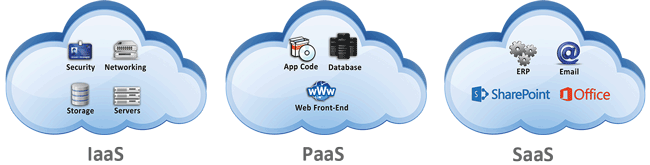
\includegraphics[width=8cm]{./service.png}
 \caption{Cloud Computing - Servcice Models \label{fig:Cloud Computing - Servcice Models} }
\end{figure}

\end{frame}

\begin{frame}{Cloud Computing - Challenges \cite{ref_1}}
Some challenges that todays Cloud Computing adopts

\begin{itemize}
\item Security
\item Costing Model
\item Charging Model
\item Service Level Agreement
\item What to migrate
\end{itemize}
\end{frame}

\begin{frame}{Cloud Computing - Deployment Model }

We can deploy the cloud in various ways.

\begin{itemize}
\item Public Cloud
\item Private Cloud
\item Hybrid cloud
\end{itemize}

\begin{figure}[H]
 \centering
 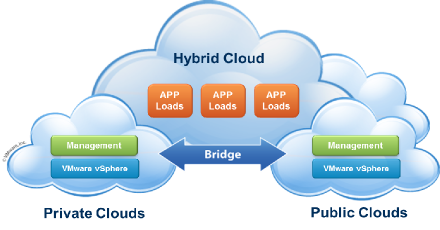
\includegraphics[width=5cm]{./model.png}
 \caption{Cloud Computing - Deployment Models \label{fig:model} }
\end{figure}
\end{frame}

\section{Private Clouds}
\begin{frame}{Private Clouds -- Introduction}

As per our concern we mainly focused about private clouds inorder to ensure Organizational data security \& High resource utilization

\hspace{4cm}\\

\textbf{``Private Cloud''} \\ 
\hspace{16mm} -- \textit{It is one of the cloud deployment model where the resources of small or medium organization are united and cattered to users of the that organization or outsourced through internet.} 

\end{frame}

\begin{frame}{Private Clouds -- Open Soruce Tools}

We can construct private cloud using some open source tools like Openstack, Cloudstack, OpenNebula. \\

\hspace{4cm} 

We can use this private cloud to deploy various services like Departmental Websites, Notice Boards, Events portal, High Computational Virtual Machines for Virtual Labs, High Performance Computing, Big data analytics.
\begin{figure}[H]
 \centering
 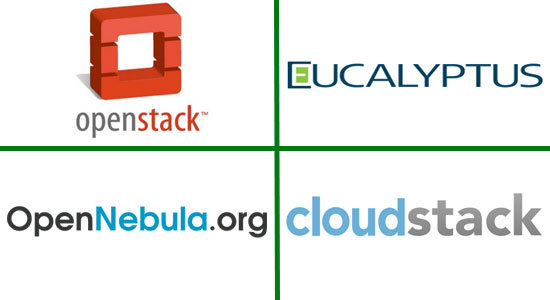
\includegraphics[width=5cm]{./cloud.jpg}
 \caption{Private Cloud - Open source tools \label{fig:cloud} }
\end{figure}

\end{frame}

\begin{frame}{Private Clouds -- Open Soruce Tools -- Comparision}

\begin{figure}[H]
 \centering
 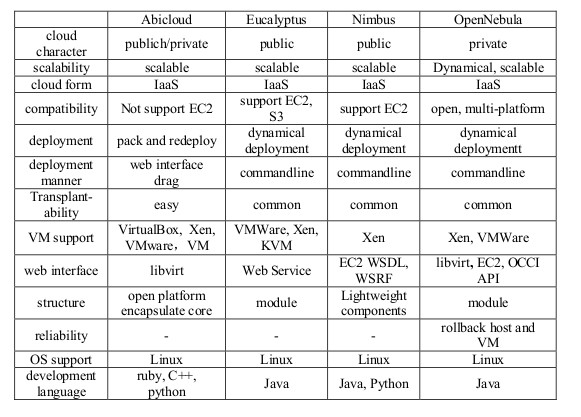
\includegraphics[width=8cm]{./comp.png}
 \caption{Open Source Tools Comparision \cite{ref_2,ref_1} \label{fig:Comparision of Open Source Tools}}
\end{figure}
\bibliography{refer}
\end{frame}

\section{Conclusion}
\begin{frame}{Conclusion}

Hardware can be effinciently utilized by tronsforming them into cloud based infra. To maintain the institutional security we are going for privte clouds. We want to go with open source tools to maintain economically optimized.
\end{frame}

\section{References}
\begin{frame}{References}
	\bibliographystyle{plainnat}
	\bibliography{my}  
\end{frame}

\end{document}